\begin{enumerate}[label=\thesubsection.\arabic*.,ref=\thesubsection.\theenumi]
\numberwithin{equation}{enumi}
\numberwithin{figure}{enumi}

\item Using Nyquist criterion, find out whether the following is stable or not.

\begin{equation}
    G(s) = \frac{100(s+5)}{s(s^2+4)(s+3)}
\end{equation}
\begin{equation}
    H(s) = 1
\end{equation}

\solution
Open loop transfer function (oltf):
\begin{equation} \label{eq:1}
    G(s)H(s) = \frac{100(s+5)}{s(s^2+4)(s+3)}
\end{equation}

Closed loop transfer function (cltf):
\begin{equation} \label{eq:2}
    \frac{G(s)}{1+G(s)H(s)}
\end{equation}

Nyquist Stability Criterion can be expressed as:
\begin{equation} \label{eq:3}
    Z = N + P
\end{equation}

where:
\begin{itemize}
    \item  Z = zeros of $ {1+G(s)H(s)}$  in RHS of s-plane 
\end{itemize}
\begin{itemize}
    \item N = number of encirclement of critical point 1+0$j$ in the clockwise direction.
    \item P = poles of G(s)H(s) in RHS of s-plane.
\end{itemize}
The pole-zero plot of equation (\ref{eq:1}) is fig. (\ref{fig:pz}) which gives \textbf{P = 0}.
\begin{figure}[ht!]
        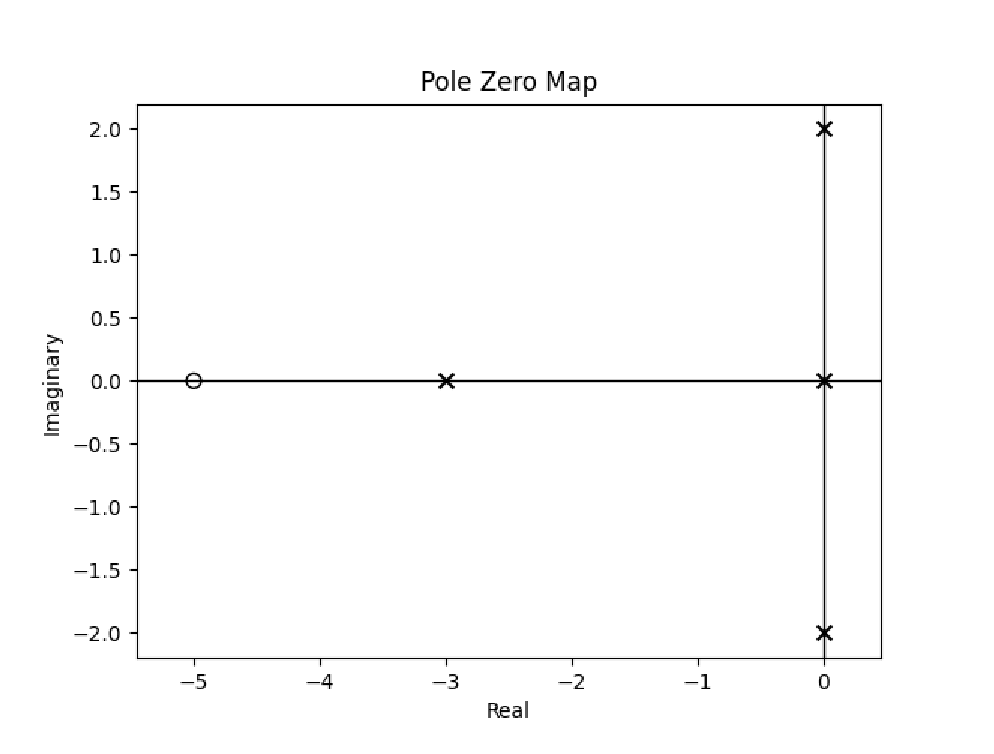
\includegraphics[width=\columnwidth]{./figs/ee18btech11025/pzG.eps}
        \caption{}
        \label{fig:pz}
\end{figure}
\begin{itemize} \label{skjvn}
    \item Since the multiplicity of zero pole is 1 (fig.\ref{fig:pz}), it should be assumed that the phasor travels one time clockwise along a semicircle of infinite radius.
    \item Same applies for poles at 2$j$ and -2$j$.
    \item Fig. (\ref{fig:splane}) shows a schematic, the dotted lines are infinite radii semi-circles.
\end{itemize}

\begin{figure}[ht!]
    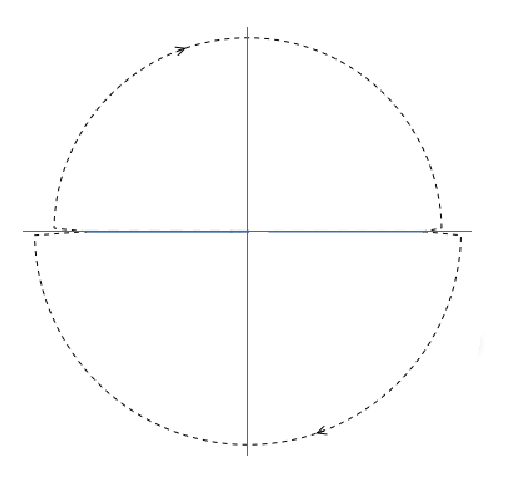
\includegraphics[width=\columnwidth]{./figs/ee18btech11025/infi.eps}
    \caption{}
    \label{fig:splane}
\end{figure}


\begin{figure}[ht!]
    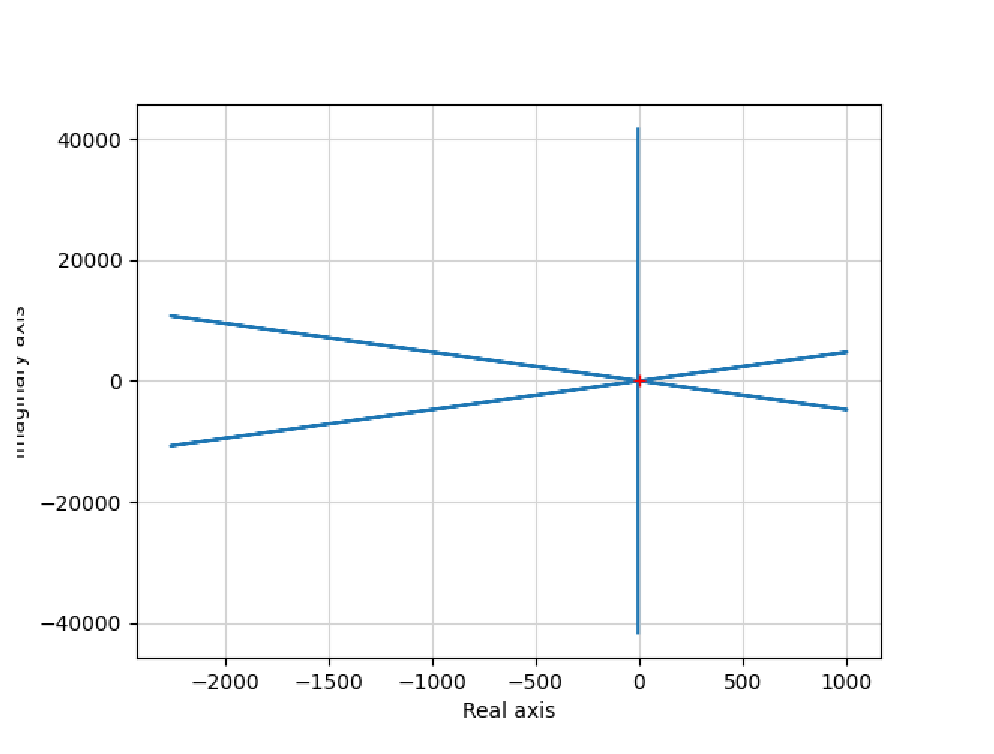
\includegraphics[width=\columnwidth]{./figs/ee18btech11025/g.eps}
    \caption{Nyquist plot of G(s)H(s)}
    \label{fig:nyqplot}
\end{figure}

\begin{figure}[ht!]
    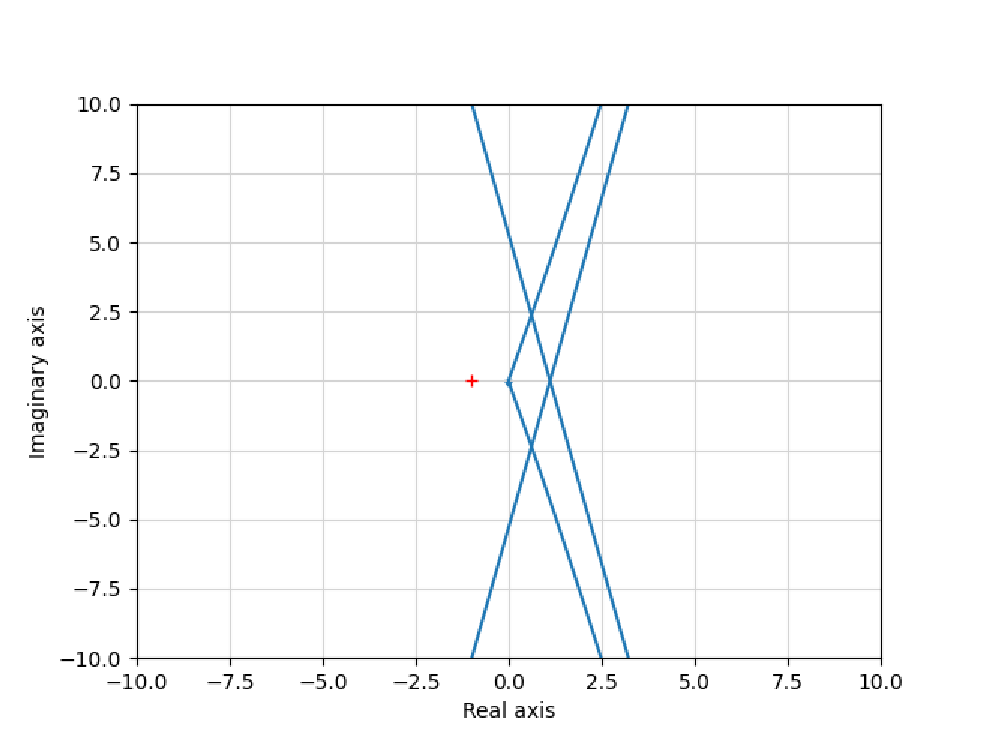
\includegraphics[width=\columnwidth]{./figs/ee18btech11025/g2.eps}
    \caption{Zoomed in}
    \label{fig:nyqplot1}
\end{figure}
\begin{itemize}
    \item The point -1+0j is not encircled by the nyquist plot (fig. \ref{fig:nyqplot1}).
\end{itemize}
From the nyquist plot (fig. \ref{fig:nyqplot1}), -1+0$j$ is not encircled by the plot. 
So from above points, the only clockwise encirclement is considered due to the mentioned poles (zero, 2$j$ and -2$j$)  with multiplicity of 1. \\  
Therefore, \textbf{N=2}

Substituting values of P = 0 and N = 2 in equation (\ref{eq:3}):
\begin{equation}
 \implies Z = 2
\end{equation}
This is verified using pole zero plot of 1+G(s)H(s) (fig. \ref{fig:pz1}).
\begin{figure}[ht!]
    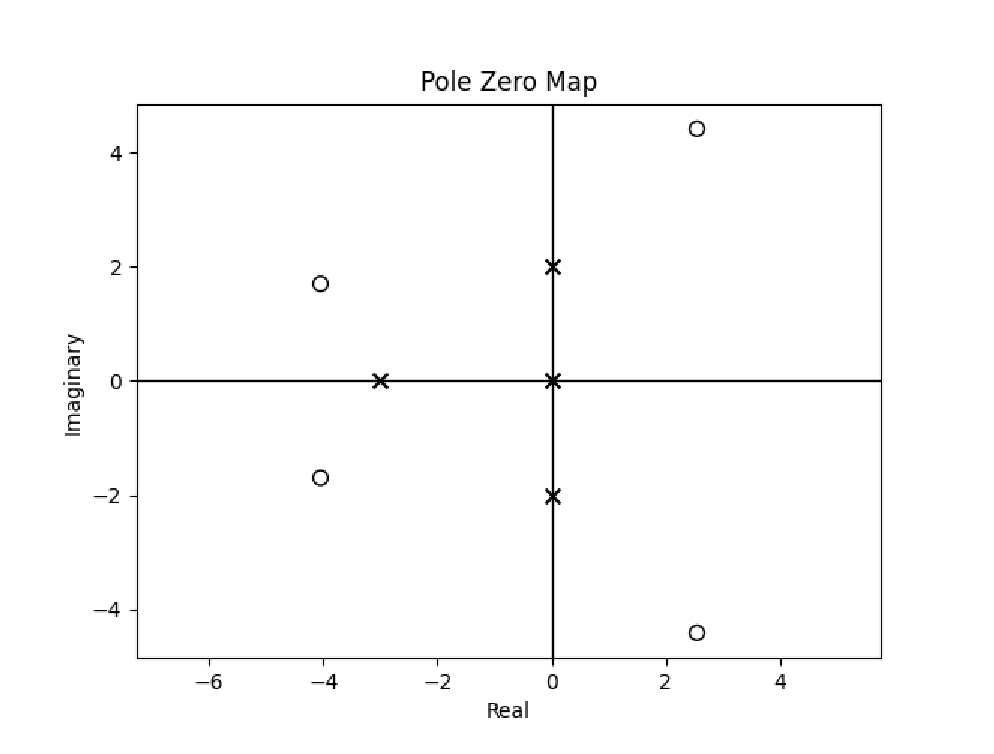
\includegraphics[width=\columnwidth]{./figs/ee18btech11025/pzG1.eps}
    \caption{}
    \label{fig:pz1}
\end{figure}
Two zeroes on RHS of s-plane i.e. Z=2. \\
Since $Z\neq0$, \textbf{the closed loop system is unstable}. \\
The \textbf{open loop system is stable} as there are \textbf{no poles on RHS} of s-plane.

The following code plots the pole zero plot and the nyquist plot.
\begin{lstlisting}
    codes/ee18btech11025.py
\end{lstlisting}
\end{enumerate}